\documentclass[english,11pt,twocolumn]{article}
\usepackage[utf8]{inputenc}  

\usepackage[english]{babel} 
\usepackage[T1]{fontenc}
%\usepackage{fullpage}
\usepackage[]{bbm}
\usepackage{amsfonts}
\usepackage{amsmath}
\usepackage{amssymb}
\usepackage{amsthm}
\usepackage{graphicx}
%\usepackage{pstricks}
\usepackage{float}
\usepackage[autolanguage]{numprint}
\usepackage[affil-it]{authblk}
%\usepackage[squaren,Gray]{SIunits}
%\usepackage{tikz}
%
%\usepackage[style=numeric,backend=bibtex]{biblatex}
\pagestyle{myheadings}


\title{Storing messages with multipartite neural cliques}
\author[]{Nissim Zerbib}
\affil{Département d'Informatique, École normale supérieure, Paris, France}

\author[]{Vincent Gripon}
\affil{Département d'Électronique, Télécom Bretagne, Brest, France}

\author{?}

\date{
	}
%

\renewcommand{\le}{\leqslant}
\renewcommand{\epsilon}{\varepsilon}
\renewcommand{\Re}{\textrm{Re}}
\renewcommand{\ge}{\geqslant}
%\newcommand{\sgn}{\textrm{le signe de }}
\newcommand{\E}{\mathcal{E}}
\newcommand{\V}{\vect{\mathcal{V}}}
\newcommand{\R}{\mathbb{R}}
\newcommand{\Z}{\mathbb{Z}}
\newcommand{\z}[1]{\Z/#1\Z}
\renewcommand{\P}{\mathbb{P}}
\newcommand{\Q}{\mathbb{Q}}
\newcommand{\N}{\mathbb{N}}
\newcommand{\C}{\mathbb{C}}
\newcommand{\U}{\mathbb{U}}
\newcommand{\f}{\widehat{f}}
\newcommand{\e}[1]{e^{-2 \pi i #1}}
\newcommand{\ex}[1]{e^{2 \pi i #1}}
\renewcommand{\L}[1]{L^{#1} (\R )}
\newcommand{\leg}[2]{\left(\dfrac{#1}{#2}\right)}

\newcommand{\vect}[1]{\overrightarrow{#1}}
\newcommand{\disp}[1]{\displaystyle{#1}}

\setcounter{secnumdepth}{3} %pour la numérotation subsubsection
\setcounter{tocdepth}{3} %pour la numérotation dans la table de matières
\renewcommand{\theenumi}{\roman{enumi})}
\renewcommand{\thepart}{\Alph{part}}
%\renewcommand{\thechapter}{\arabic{chapter}}
\renewcommand{\thesection}{\Roman{section}}
\renewcommand{\thesubsection}{\arabic{subsection}}
\renewcommand{\thesubsubsection}{\alph{subsubsection}}

\newcommand{\fonction}[5]{\begin{array}{cllll}
#1 & : & #2 & \longrightarrow & #3 \\
&    & #4 & \longmapsto & #5 \end{array}}
\newcommand{\fonc}[3]{\begin{array}{lllll}
#1: & #2 & \mapsto & \displaystyle{#3}\end{array}}
\newcommand{\app}[3]{
	#1 : #2 \mapsto \displaystyle{#3}}
\newcommand{\fonct}[3]{\begin{array}{ccccc}
#1: & #2 & \longrightarrow & \displaystyle{#3}\end{array}}
\newcommand{\pent}[1]{\lfloor #1 \rfloor}

% Le point-virgule bien espacé
\newcommand{\pv}{\ensuremath{\, ; }}
% Les intervalles
   % fermé - fermé
   \newcommand{\interff}[2]{\ensuremath{\left[ #1 \pv #2 \right]}}
   % fermé - ouvert
   \newcommand{\interfo}[2]{\ensuremath{\left[ #1 \pv #2 \right[}}
   % ouvert - fermé
   \newcommand{\interof}[2]{\ensuremath{\left] #1 \pv #2 \right]}}
   % ouvert - ouvert
   \newcommand{\interoo}[2]{\ensuremath{\left] #1 \pv #2 \right[}}


\theoremstyle{definition}
\newtheorem{theoreme}{Theorem}
\renewcommand{\thetheoreme}{\arabic{section}.\arabic{theoreme}}
\providecommand{\keywords}[1]{\textbf{Index terms---} #1}

\newcommand{\comp}[3]{\left\{
	#1\,;\, #1\in #2 \, /\, #3
	\right\}}
\newcommand{\param}[2]{\left\{
	#1\, /\, #2
	\right\}}


\begin{document}

	\maketitle

	 \begin{abstract}
	 	We extend recently introduced associative memories based on cliques to multipartite cliques. We propose a variant of the classic retrieving rule. We study their relative performance for retrieving partially erased and corrupted messages. We provide both analytical and simulation results showing improvements of capacity over.
	 \end{abstract}
	 
	\keywords{associative memory, error correcting code, cliques, multipartite cliques, neural networks}
	
	\section{Introduction}
	
		
	
	\section{Networks of neural cliques}
		
	\subsection{Learning messages}
	
	\subsection{Retrieving messages}	
	
		\subsubsection{The "winner takes all" rule}	
	
		\subsubsection{The "$a$ winners take all" rule}
		
		less biologically plausible rule
		
		same algorithmic complexity
	

	\section{Retrieval performance}	
	

	\subsection{Retrieving partially erased messages}		
		
	\subsubsection{Analytical result}
		
	number of neurons per cluster $l$
	
	number of clusters $c$
	
	number of erased clusters $c_e$
	
	number of messages : $m$
	
	number of activities per cluster : $a$
	
	density : $d$

	edge : $(i, j)$
	
	As the probability for $i$ and $j$ to be active in their respective clusters for one message is $\frac{a}{l}$, providing messages are independent, it follows that the probability for the edge $(i,j)$ of not being added in the network for one message is $1 - \left(\frac{a}{l}\right)^2$. Thus the density $d$ can be expressed like this :
	
			
	\[ d = 1 - \left( 1 - \left(\frac{a}{l}\right)^2 \right)^m \]
	
	Thanks to the memory effect $\gamma$, activated neurons in a non-erased cluster stays activated and are the only ones doing so in their cluster. For neurons in erased clusters, the maximum attainable score is $a(c - c_e)$. Neurons corresponding to the original message achieve this score. Besides the probability for a neuron $v$ to achieve the maximum score in such a cluster, that is to mean $a(c-c_e)$ is $d^	{a(c-c_e)}$.
	
	probability for a vertex $v$	not to achieve the maximum : $1 - d^	{a(c-c_e)}$
	
	Since neurons representing messages are independent (as messages are themselves independent), the probability for none of the vertices of one erased cluster, excepting the correct ones, to achieve the maximum is $\left(1 - d^	{a(c-c_e)}\right)^{l-a}$.
	
	Scores in clusters being also independent, the probability for none of the vertices in any erased cluster, excepting the correct ones, to achieve the maximum in their respective clusters is $\left(1 - d^	{a(c-c_e)}\right)^{c_e(l-a)}$.
	
	Whence error rate in retrieving messages is : \[P_{err} = 1 -	\left(1 - d^	{a(c-c_e)}\right)^{c_e(l-a)} \]
	
	
	$\eta_m = (P_{retrieve} m ) \frac{2 \left(c \log_2{l \choose a } - \log_2(m) + 1 \right)}{c(c-1)l^2} \times \frac{c}{(c-c_e) \log_2{l \choose a }}$
	
	$\eta_{max} = \max_x \eta_x $
	
	\subsubsection{Simulations}
		gap of theoretical density with density in simulations : under $1$ percent
		
		New rule : Improves the retrieval rate for multiple iterations and/or corrupted messages.
		
		The simulations agree with the analytical results for density and error rate.
	

	For one iteration (for erasures, not for errors), winner takes all is the same as $a$-winners take all.
	
	For multiple iterations $a$-winners take all is a significant improvement.
	
		"$a$-winners take all" better than "winner takes all" with errors instead of erasures, even for one iteration.
	
	For errors : only better than only 1 activity per cluster if multiple iterations of the $a$-winners take all rule.
	For one iteration, it is less efficient.
	\begin{figure}
		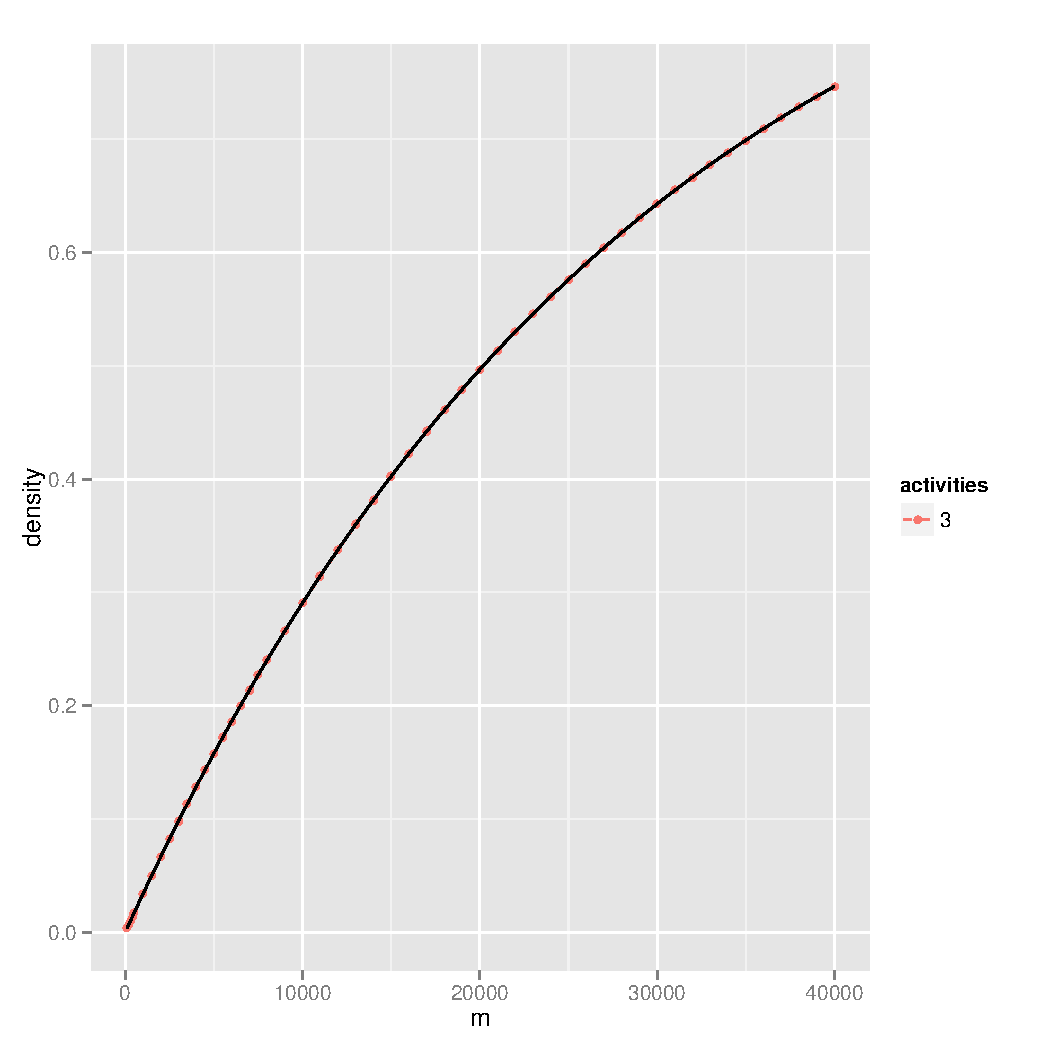
\includegraphics[width=8.5cm]{Courbes/densiteexemple.pdf}
		\caption{Theoretical and empirical densities}
	\end{figure}
	
	\begin{figure}
		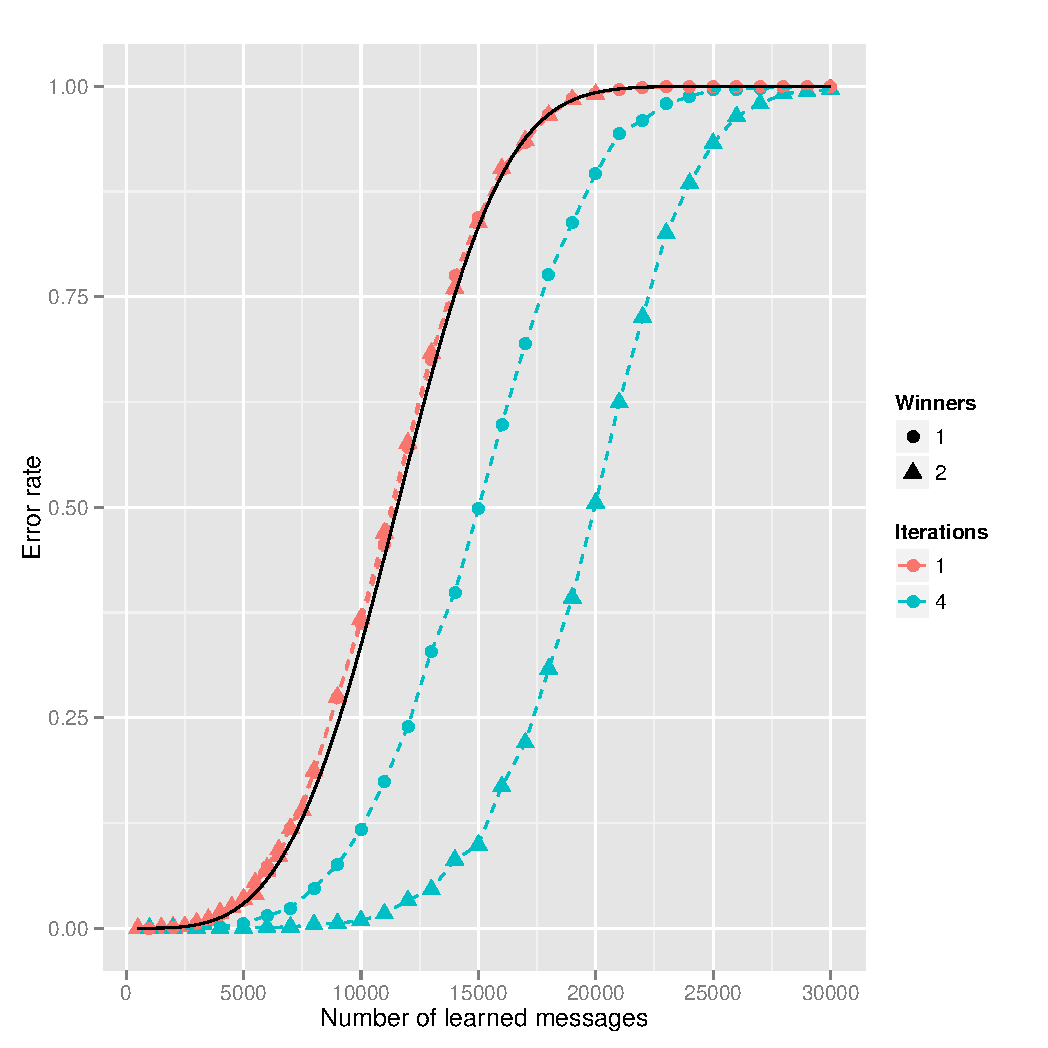
\includegraphics[width=8.5cm]{Courbes/remplacement_figure2g1} %{comparaison_regles_pool5_a2c4l512e2}
		\caption{2 activities per cluster, 4 clusters, 512 neurons per cluster, two erasures, each point is the mean of 5 networks with 1000 sampled messages, analytical result in continuous black}
		\end{figure}
			
	\newpage
	p
	\newpage
	
	\subsection{Retrieving corrupted messages}
	\begin{figure}
		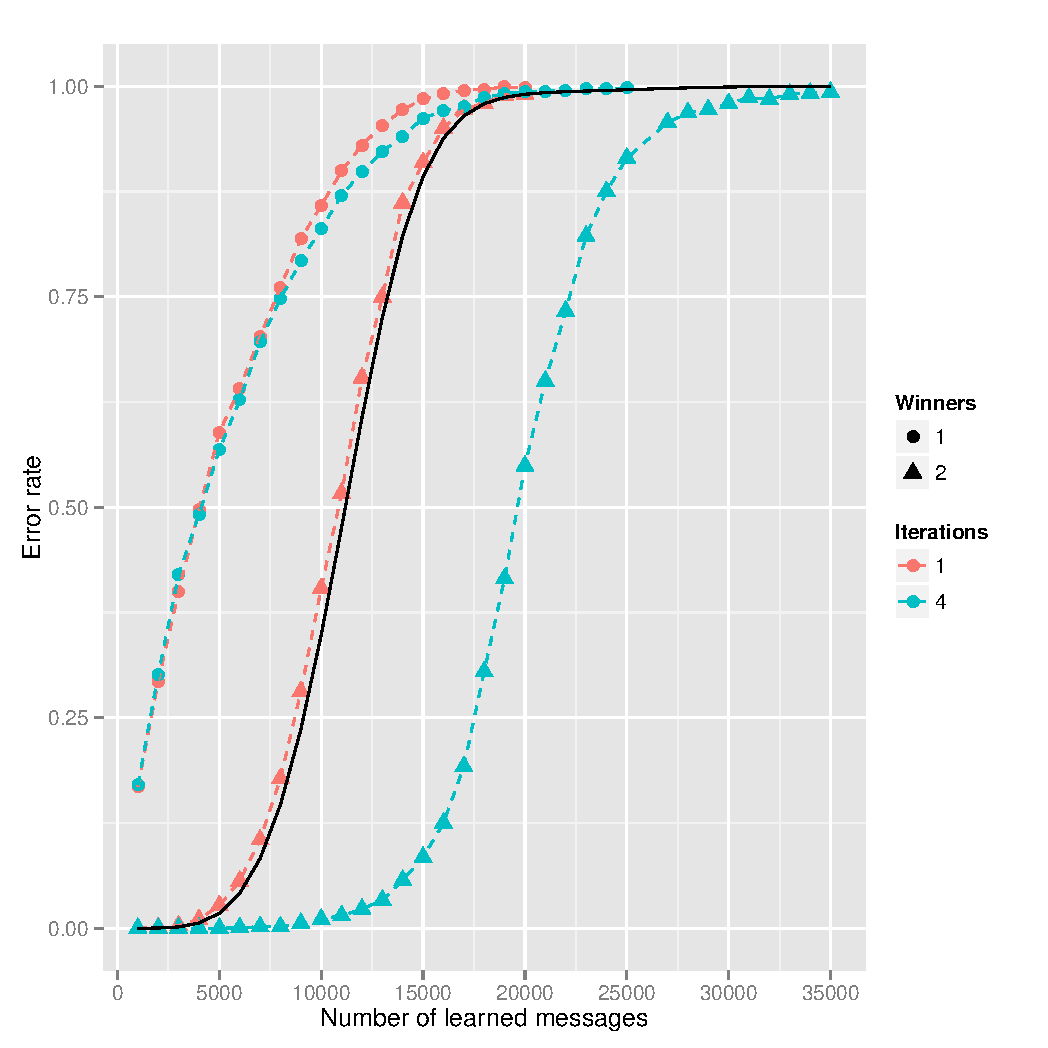
\includegraphics[width=8.5cm]{Courbes/remplacement_figure3g1}
		\caption{2 activities per cluster, 4 clusters, 512 neurons per cluster, one erroneous cluster, each point is the mean of 5 networks with 1000 sampled messages, analytical result in continuous black}
	\end{figure}
		
		
		\begin{figure}
		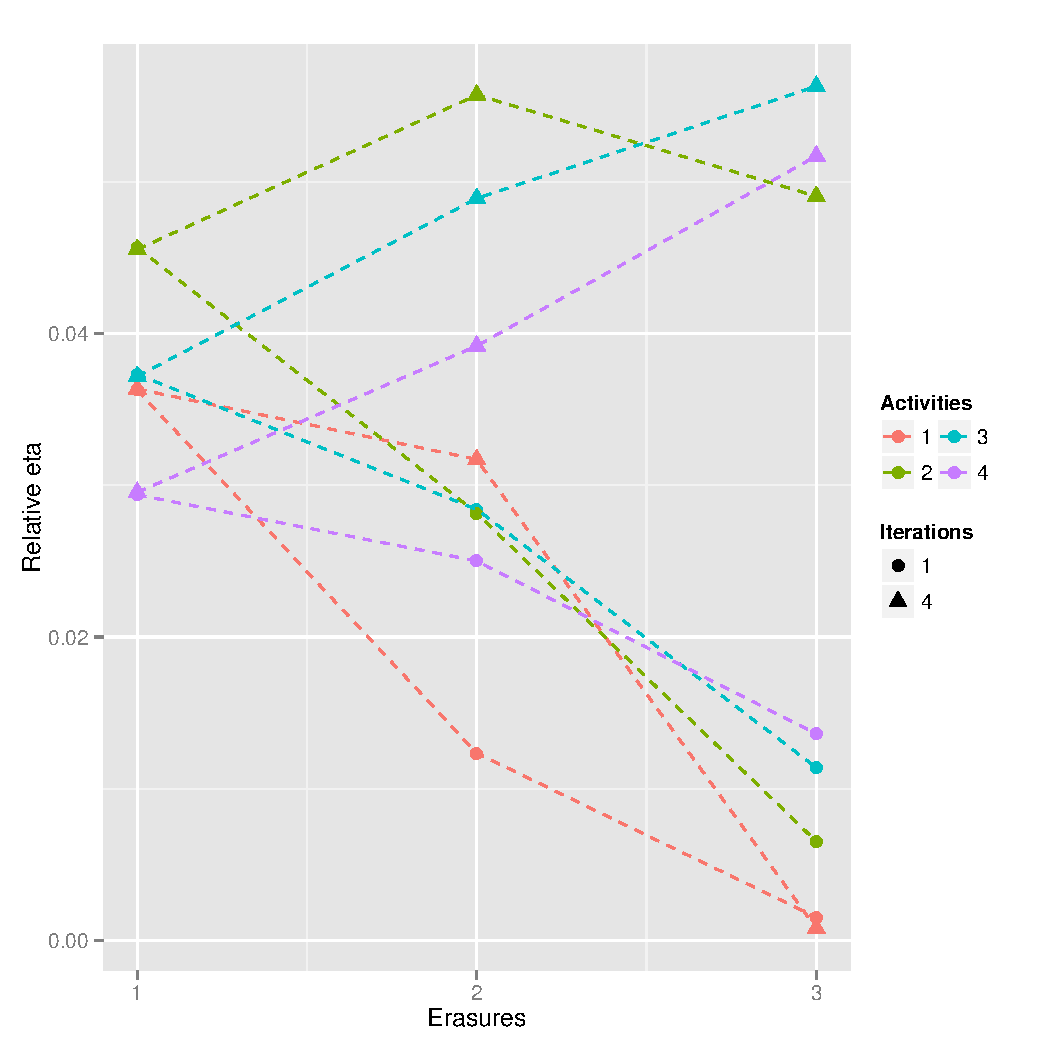
\includegraphics[width=8.5cm]{Courbes/remplacement_figure4g1}
		\caption{Comparison between different number of activities per cluster :  4 clusters, 512 neurons per cluster, 1000 sampled messages}
	\end{figure}
		

	
	
	Formula for errors instead of erasures : 
	
	gc : good (à remplacer par right/wrong ?) neuron in correct cluster
	
	ge : good neuron in erroneous cluster
	
	abe : bad activated neuron in erroneous cluster
	
	be : others bad (à remplacer par wrong ou incorrect etc.) neurons in erroneous cluster
	
	bc : bad neuron in correct cluster
	
	$P(n_{gc} = (c - c_e - 1) + \gamma + x) = {c_e \choose x} d^x (1-d)^{ce-x}$
	
	$P(n_{ge} = (c - c_e) + x) = {c_e - 1 \choose x} d^x (1-d)^{c_e-1-x}$
	
	$P(n_{abe} = \gamma + x) = {c - 1 \choose x} d^x (1-d)^{c-1-x}$
	
	$P(n_{be} = x) = P(n_{bc} = x) = {c - 1 \choose x} d^x (1-d)^{c- 1 -x}$
	
	
	
	$
	P_{retrieve} = \left [ \sum_{n = 1}^{c-1+\gamma} P(n_{gc} = n) \left [ \sum_{x=0}^{n-1} P(n_{bc} = x) \right]^{l-1} \right ]^{c - c_e} \\ \times \left [ \sum_{n = 1}^{c-1+\gamma} P(n_{ge} = n) \left [ \sum_{x=0}^{n-1} P(n_{bc} = x) \right]^{l-2} \left [ \sum_{x=0}^{n-1} P(n_{abc} = x) \right] \right ]^{c_e}
	$
	
	%à changer : prendre en compte les $a$ neurones activés : problème des recouvrements !! on est trop optimiste si grand nombre d'activités (ou pessimiste ?)
	
	generalisation to multiple activities per cluster :
	\newpage
	$\,$
	\newpage
	
	$P(n_{gc} = a(c - c_e - 1) + \gamma + x) = {a c_e \choose x} d^x (1-d)^{a ce-x}$
	
	$P(n_{ge} = a(c - c_e) + x) = {a (c_e - 1) \choose x} d^x (1-d)^{a (c_e - 1)-x}$
	
	$P(n_{abe} = \gamma + x) = {a(c - 1) \choose x} d^x (1-d)^{a(c-1)-x}$
	
	$P(n_{be} = x) = P(n_{bc} = x) = {a(c - 1) \choose x} d^x (1-d)^{a(c- 1) -x}$	

	
	
	%\begin{align*}
	$P_{retrieve} = \left [ \sum_{n = 1}^{a(c-1) + \gamma} \left [ \sum_{k = 1}^{a} { a \choose k }   P(n_{gc} = n)^k P(n_{gc} > n)^{a-k} \right ] P(n_{bc} < n)^{l-a} \right ]^{c - c_e} \\ \times \left [ \sum_{n = 1}^{a(c-1) +\gamma} \left[ \sum_{k = 1}^a { a \choose k } P(n_{ge} = n)^k P(n_{ge} > n)^{a-k} \right ] P(n_{bc} < n)^{l-2a} P(n_{abc} < n)^a \right ]^{c_e}
	$
	%\end{align*}
	
	$P_{err} = 1 - P_{retrieve}$
	
	\newpage
	$\,$
	\newpage
	
	\section{Conclusion}	
	
	
	
	%Marche mieux pouur de petits c --> le faire sur le sparse ?
	
	\section{Resilience}
	Spéculations en Français :
	
	Peut-être un intérêt pour cluter based associative memories build from unreliable storage : si une arête porte moins d'info, on peut peut-être en supprimer plus (mais rajout ?!)
	

	Marche mieux pour des bruits importants
	
	$P(n_{v_c} = n_0) = {a c_k \choose n_0} (1-\psi)^{n_0} \psi ^ { a c_k - n_0 }$
	
	$P_+ = \psi (1 - d) + (1 - \psi) d$
	
	$P(n_v = x) = {a c_k \choose x} P_+^x (1-P_+)^{a c_k -x }$

	% À corriger avec sommes multiparties
	%$P(\mbox{no other vertex activated in this cluster})= \sum_{n_0 = 1}^{a (c - c_e)} P(n_{v_c} \ge n_0)^a \left [ \sum_{x = 0}^{n_0 - 1} P(n_v = x) \right]^{l-a}$
	
	%$P(\mbox{no other vertex activated in any cluster})=  \left ( \sum_{n_0 = 1}^{a ( c - c_e)} P(n_{v_c} \ge n_0)^a \left [ \sum_{x = 0}^{n_0 - 1} P(n_v = x) \right]^{l-a } \right)^{c_e}$
	
	Sans tenir compte du choix au hasard si plus sont activés.
	
		a priori for noise on edges :

	$P(\mbox{no other vertex activated in this cluster})= \sum_{n = 1}^{a (c - c_e)} \left [ \sum_{k = 1}^{a} { a \choose k }   P(n_{v_c} = n)^k P(n_{v_c} > n)^{a-k} \right ] \left [ \sum_{x = 0}^{n - 1} P(n_v = x) \right]^{l-a }$
	
	$P(\mbox{no other vertex activated in any cluster})=  \left ( \sum_{n = 1}^{a ( c- c_e)} \left [ \sum_{k = 1}^{a} { a \choose k }   P(n_{v_c} = n)^k P(n_{v_c} > n)^{a-k} \right ] \left [ \sum_{x = 0}^{n - 1} P(n_v = x) \right]^{l-a } \right)^{c_e}$	
	
	\newpage
	$\,$
	\newpage
	\begin{figure}
		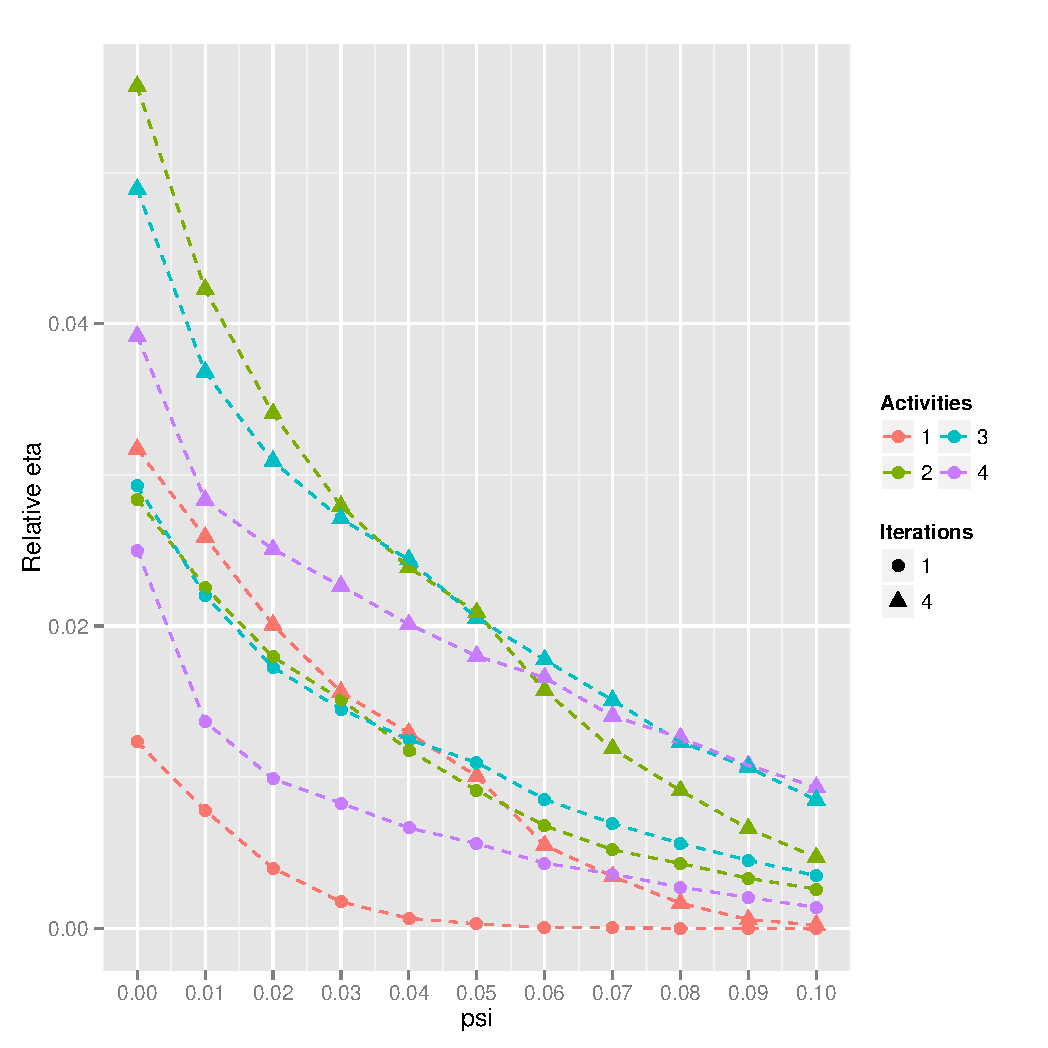
\includegraphics[width=8.5cm]{Courbes/1comppsic4l512g1}
		\caption{Comparison between different number of activities per cluster :  4 clusters, 512 neurons per cluster, 1000 sampled messages}
	\end{figure}

	
	
	\nocite{*}
	\bibliographystyle{numeric} % Le style est mis entre crochets.
         \bibliography{bibli.bib}
\end{document}
